%%
%% This is file `sample-sigconf.tex',
%% generated with the docstrip utility.
%%
%% The original source files were:
%%
%% samples.dtx  (with options: `sigconf')
%% 
%% IMPORTANT NOTICE:
%% 
%% For the copyright see the source file.
%% 
%% Any modified versions of this file must be renamed
%% with new filenames distinct from sample-sigconf.tex.
%% 
%% For distribution of the original source see the terms
%% for copying and modification in the file samples.dtx.
%% 
%% This generated file may be distributed as long as the
%% original source files, as listed above, are part of the
%% same distribution. (The sources need not necessarily be
%% in the same archive or directory.)
%%
%% The first command in your LaTeX source must be the \documentclass command.
\documentclass[sigconf]{acmart}
\usepackage[noend]{algpseudocode}
\usepackage{algorithm}
\usepackage{booktabs}
\usepackage{subfig}

\usepackage{xcolor}
\usepackage[linesnumbered,ruled,vlined]{algorithm2e}

%%
%% \BibTeX command to typeset BibTeX logo in the docs
\AtBeginDocument{%
  \providecommand\BibTeX{{%
    \normalfont B\kern-0.5em{\scshape i\kern-0.25em b}\kern-0.8em\TeX}}}

%% Rights management information.  This information is sent to you
%% when you complete the rights form.  These commands have SAMPLE
%% values in them; it is your responsibility as an author to replace
%% the commands and values with those provided to you when you
%% complete the rights form.
\setcopyright{acmcopyright}
\copyrightyear{2018}
\acmYear{2018}
\acmDOI{10.1145/1122445.1122456}


%% These commands are for a PROCEEDINGS abstract or paper.
\acmConference[Woodstock '18]{Woodstock '18: ACM Symposium on Neural
  Gaze Detection}{June 03--05, 2018}{Woodstock, NY}
\acmBooktitle{Woodstock '18: ACM Symposium on Neural Gaze Detection,
  June 03--05, 2018, Woodstock, NY}
\acmPrice{15.00}
\acmISBN{978-1-4503-XXXX-X/18/06}



%%
%% Submission ID.
%% Use this when submitting an article to a sponsored event. You'll
%% receive a unique submission ID from the organizers
%% of the event, and this ID should be used as the parameter to this command.
%%\acmSubmissionID{123-A56-BU3}

%%
%% The majority of ACM publications use numbered citations and
%% references.  The command \citestyle{authoryear} switches to the
%% "author year" style.
%%
%% If you are preparing content for an event
%% sponsored by ACM SIGGRAPH, you must use the "author year" style of
%% citations and references.
%% Uncommenting
%% the next command will enable that style.
%%\citestyle{acmauthoryear}

%%
%% end of the preamble, start of the body of the document source.
\begin{document}

%%
%% The "title" command has an optional parameter,
%% allowing the author to define a "short title" to be used in page headers.
\title{DeepBugs: A Learning Approach to Name-Based Bug Detection}

%%
%% The "author" command and its associated commands are used to define
%% the authors and their affiliations.
%% Of note is the shared affiliation of the first two authors, and the
%% "authornote" and "authornotemark" commands
%% used to denote shared contribution to the research.
\author{Iman Chatterjee}
\authornote{Both authors contributed equally to this research.}
\affiliation{%
  \institution{UC Davis}
  \city{Davis}
  \state{California}
}
\email{imnchatterjee@ucdavis.edu}

\author{Lakhveer Kaur}
\affiliation{%
  \institution{UC Davis}
  \streetaddress{1 Th{\o}rv{\"a}ld Circle}
  \city{Davis}
  \state{California}}
\email{lvkaur@ucdavis.edu}





%%
%% By default, the full list of authors will be used in the page
%% headers. Often, this list is too long, and will overlap
%% other information printed in the page headers. This command allows
%% the author to define a more concise list
%% of authors' names for this purpose.
\renewcommand{\shortauthors}{Trovato and Tobin, et al.}

%%
%% The abstract is a short summary of the work to be presented in the
%% article.
\begin{abstract}
Automatic Bug detection is a critical strategy that helps saves a lot of the developer's time. A few popular ways to perform bug detection are genetic programming, machine learning and pattern matching. DeepBugs paper uses machine learning path to train three model where each can predict a specific kind of bug. In this paper, we extend the DeepBugs to train two more models. These models will find Wrong Return Statement bug and Empty Block Statement bug. We create a training data from the given corpus with new bugs. Models trained on newly created data, are capable of predicting the same bug in an unseen code. The new models was trained on a large corpus of 150,000 JavaScript files respectively to obtain the promising accuracies of 71\% and 91\% respectively on the Wrong Return Statement and Empty Block Statement bugs detectors.
\end{abstract}

%%
%% The code below is generated by the tool at http://dl.acm.org/ccs.cfm.
%% Please copy and paste the code instead of the example below.
%%
\begin{CCSXML}
<ccs2012>
<concept>
<concept_id>10011007.10011006</concept_id>
<concept_desc>Software and its engineering~Software notations and tools</concept_desc>
<concept_significance>500</concept_significance>
</concept>
<concept>
<concept_id>10011007.10011074.10011099</concept_id>
<concept_desc>Software and its engineering~Software verification and validation</concept_desc>
<concept_significance>500</concept_significance>
</concept>
<concept>
<concept_id>10010147.10010257.10010293.10010294</concept_id>
<concept_desc>Computing methodologies~Neural networks</concept_desc>
<concept_significance>500</concept_significance>
</concept>
</ccs2012>
\end{CCSXML}

\ccsdesc[500]{Software and its engineering~Software notations and tools}
\ccsdesc[500]{Software and its engineering~Software verification and validation}
\ccsdesc[500]{Computing methodologies~Neural networks}


%%
%% Keywords. The author(s) should pick words that accurately describe
%% the work being presented. Separate the keywords with commas.
\keywords{Bug detection, Natural language, Machine learning, Name-based program
analysis, JavaScrip}

\maketitle

\section{Introduction}
A name-based analysis must reason about the meaning of identifier names. As a form of natural language information, identifier names are inherently fuzzy and elude the precise reasoning . Thus, most existing bug detection tools ignore vital information such as names of variables and function and tend to miss some classes of potential bugs.
The few existing name-based bug detection approaches reason about names on a syntactic level and rely on manually designed and tuned algorithms to detect bugs.  Source code provides a lot of useful insight on the semantics and natural language information. Most typical program analysis methodologies tend to ignore identifier names or the contents of conditional blocks although many of these can contain potential bugs. Ignoring these can cause bug analysers to skip bugs that are glaringly obvious to the human eye.
\newline In spite of an increasing requirement that software be reliable, program bugs keep appearing frequently. Non-stop systems having stringent uptime requirements \cite{hangal} need to be kept running even when there is a risk of hardware or software failure. Such systems have a critical need for a mechanism to automatically monitor, debug and fix bugs on the fly. Use of incorrect intermediate results due to undetected bugs can have a catastrophic effect in systems that are mission-critical or even safety-critical.Also, human programmers are often careless in documenting the specifications for the software in detail. Thus bugs arising in such systems, especially those that arise in corner cases can take upto weeks to debug. Human debugging time can greatly be reduced  through techniques for automatic bug detection. 
\newline DeepBugs is an automatic bug detection approach that is based on the names of variables or functions. The basic principle is to train a classifier to distinguish between code that is an instance of a name-related bug pattern and code that does not suffer from this bug pattern. Bug patterns refer to a class of programming errors that are similar because they violate the same rule. Since the name of a function describes a lot about its body, and helps in  finding bugs more accurately, feeding a program to Deepbug detector,  tells whether or not a program is buggy. None of the existing automatic bug detection programs before Deepbugs were taking the function/program names into account.
\newline DeepBugs uses a machine learning-based approach. A learned vector representation of identifiers called 'embeddings' preserves semantic similarities, such as the fact that length and count are similar.  The problem is formulated as a binary classification and a model is trained to distinguish correct code from incorrect code. 
\newline The approach uses a feedforward neural network with an input layer of a size that depends on the code representation provided by the specific bug detector, a single hidden layer of size 200, and an output layer with a single element that represents the probability computed by the detector. A dropout of 0.2 is applied to the input layer and the hidden layer. Binary cross-entropy is used as the loss function and RMSprop optimizer is used to train the network for 10 epochs with a batch size of 100.
\newline Because the classifier is learned without human intervention,the approach does not rely on designing and tuning heuristics. We have added two more bug detectors to the existing system for an incorrect return value and for missing block or empty statements in block. Lakhveer and Iman contributed equally to the project with Lakhveer primarily working on Incorrect Return Statement and Iman working on Missing Block(or Incorrect Conditional). We have used a dataset of size 150,000 provided by Srilabs(\underline{\href{https://www.sri.inf.ethz.ch/js150}{https://www.sri.inf.ethz.ch/js150}}) as recommended by the author. The JavaScript programs are collected from GitHub repositories by removing duplicate files, removing project forks (copy of another existing repository), keeping only programs that parse . For parsing, the error-tolerant Acorn parser (using the parse\_dammit interface) has been used. The corpus is split into a set of 100,000 training files with a validation set of 50,000 files. We also test our model on a very small subset of this big corpus. We have named this subset as programs\_50 since it consists of 50 files with the author specifying 29 files as training files and the remaining 21 for validation.

\section{Background}
Deepbugs trained three bug detectors namely: accidentally swapped arguments in a function call, in correct binary operator and incorrect binary operand. Each bug detector can predict only one specific kind of bug. Since, Deep Bugs is trained on only three bugs so far, its capability is limited. Training more models will expand its ability to predict five kind of bugs.  
\par
In our project, we are going to train two model on bugs like incorrect return value and empty conditional statement. Incorrect return statement is a case when a programmer accidentally returns a wrong argument in a function. Below functions shows such example. From name of the function, it can be predicted that function should add two parameters, and should return the sum. However, it is returning some other value. Incorrect return statement bug detector is trained to predict such instances. 

\begin{algorithm}[H]
\caption{Sum Function for demonstrating incorrect return statement bug use case}
\begin{flushleft}

% Set Function Names
  \SetKwFunction{FMain}{Main}
  \SetKwFunction{FSum}{Sum}
  \SetKwFunction{FSub}{Sub}
 
% Write Function with word ``Function''
  \SetKwProg{Fn}{Function}{:}{}
  \Fn{\FSum{$first$, $second$}}{
        a = first\; \\
        b = second\; \\
        sum = first + second\; \\
        \KwRet a\;
  }
  \;
\end{flushleft}
\end{algorithm}


\iffalse
For example, in case of incorrect return value, buggy code can be generated from the given data set of correct codes by changing the return value in a function to something completely random, or we can replace it with some other variable from the program. To create the training example,  we will create an Abstract Syntax Tree (AST) of a code snippet like explained in the paper. Traversing through the AST, the program will extract the return type and return value.  Then will change the returned value to something else of the return type. This would give us training data to feed in a neural network. 

\fi
\par
The bug named Empty conditional statement is characterized by the presence of an empty statement after an if statement or an empty block(or compound statement) which makes the control flow statement useless since control flow would continue onto the same place regardless of whether or not the branch is taken.\newline
\newline Identification and removal of such ineffectual 'if branching' thus makes the code cleaner and more reliable.Buggy code or negative examples for incorrect if statement can be generated from the given data set of correct codes by replacing the type of the consequent to an undefined or a null type. Since such bugs where empty blocks are found after 'if statements' are very rare, we extend our use case to if blocks that contain one or more 'empty statements' in the consequent. 
\begin{figure}[h!]
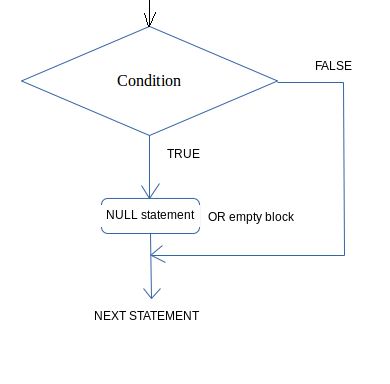
\includegraphics[width=50mm]{untitled(2).png}
\caption{Example of a conditional block with an empty statement}
\end{figure}
As evident from figure 1, if the consequent or the statement in the body of the 'if true' section of the conditional expression is a null statement(which could be characterized by an empty block or empty statements(semicolons),the control automatically moves to 'Next statement' which would have also have been the first statement to be executed if the condition had evaluated to 'false'. So we see that even in the absence of such a branching conditional expression, 'Next statement' would have been executed. 
Presence of empty statements and empty blocks following conditional expressions thus contribute to unnecessary redundancy and lead to situations where the same code is executed regardless of whether the 'if' or 'else' path is taken. 
\newline An example of how the AST for incorrect if statement looks is provided in Figure 2. In the figure we also see that a null statement was found inside one of our conditional expressions. Such cases cannot be handled using the DeepBugs implementation developed by the author.Hence the need for a new bug detector for incorrect if statement. 
\begin{figure}[h!]
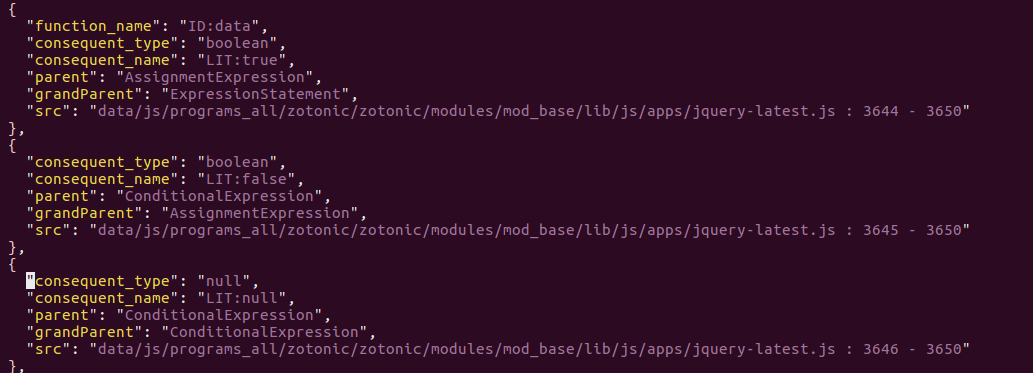
\includegraphics[width=100mm]{untitled(4).png}
\caption{Example of a null statement containing a null literal}
\end{figure}
\newline An example of a situation where 'incorrect return statement' bug may arise would be a case where a summing function expected to return a numeric value c(the sum of input parameters a and b) ends up returning some unexpected integer value(a,b or some other random value). While this situation would not cause an exception, it would affect all the subsequent execution stages. Since the existing implementation of DeepBugs has no provision for handling bugs like this, we  have developed our own bug detector to detect incorrect return statement.


\section{Technical Approach}
    In this section, we give an overview of BugDetection algorithm. We consider that finding a bug is a binary problem. Either a code snippet has a bug or it does not have a bug. Deep Bug paper decibels three type of bugs and train a model for each one. Trained model will automatically find that specific kind of bugs in an unseen code. We added two more bug types to the model. These types are: wrong return statement in a function and absence of block in an if statement. 
    The general way to train a model with any kind of bug is essentially the same. The first step is to get the training data. Deep Bugs paper have a thousands of programs taken from github \cite{pradel2018deepbugs}. Instead of finding real buggy program, We are going to use the same data set to train the new bugs. It is assumed that, at first, all the programs are bug free. We extract the code snippets related to the bug from a given program. For example, for wrong-return-statement bug, we want to focus only on parts of program where a return statement is written. For this purpose, every code snippet is parsed to an Abstract Syntax Tree (AST). By going through AST, the nodes that are related to a particular bug detector are extracted. After that, a node(s) is changed or deleted, depending upon the bug detector. For example, in Incorrect Return Statement Bug Detector, return value will be replaced with some other attribute from the program. The replaced value might not produce a syntax error but it will create a bug. In empty block statement, first, algorithm finds all entries of if-statement. Then it deletes the body of every if-statement and create a null consequent. Deleting body will create an empty block statement bug. 
    
    By putting error in code examples, we have a correct and incorrect version of a same code snippet. This creates our training data. 
    
    Second step is to change the training data into vector format. Since machine learning models work with vectors, and cannot read a code snippet itself. Code/text is required to change into numbers/vector representation. There are two main ways for this: One hot encoding, Word2vec. In this program, we are using Word2Vec. From AST, we extract the required node names. Word2Vec embed the names to series of numbers with relative words with relative numbers. DeepBugs paper used CBOW variant of Word2Vec. We are going to use the same variant for this purposes. 
    
    Third Step in the process is to train the model. By providing positive (good code) and negative (buggy code) examples, a feedforward network is trained. Machine learning model works like a black box. To increase model accuracy, multiple layers can be used. Since Machine learning models can easily over fit the data, some dropouts are used in model. Once trained, model takes an example of unseen code and produces a number between zero and one. The produced number is a probability that how likely the provided code is buggy according to model. \ref{overview}. shows the overview of DeepBugs process.
    
 
 \begin{figure*}[h!]
 \centering
  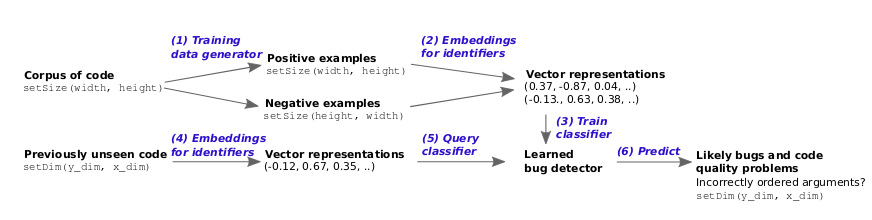
\includegraphics[width=0.8\textwidth]{DeepBugs_Overview of Approach.png}
  \caption{\small Overview of DeepBugs Approach}
  \label{overview}%
\end{figure*}
 
 
\subsection{Paper Additions} 
In DeepBugs, three models are trained for three bugs: Swapped Function Arguments, Wrong Binary Operator, Wrong Binary Operand in Binary Operation. For any new code, trained Deep Bugs model can identify only these specific bugs. For example, Swapped Functions model will specify whether or not a program has a bug caused by accidentally swapped arguments. Note that, this specific model will not predict any other bug. In this paper, we added two more model bugs that DeepBugs can predict. 

This paper uses the Deep Bugs as a base. Since every model is pruned to a specific, it captures only specif keywords from a program to find bug. For example, swapped arguments detector scans  arguments and parameters of a function and discards everything else. This paper added two more detectors. First, wrong return statements, which captures returned argument of a function. The code implementation can be found in extractorOfRetVal.js in JavaScript folder. Second, empty block statements bug detector, captures consequent of an if-statement in a program. Implementation for empty block statement can be found in extractorOfConditions.js in JavaScript folder. 

 Since each model is trained separately on a specific bug, it has its own data set. Data set should contain both positive and negative examples. By capturing the necessary data from given code, we already have a positive example. Each bug detector has its own format to introduce a bug and create a negative example. For example, swapped arguments detector swapped both arguments in a function call to create a bug. This paper adds negative examples for newly introduced bug detector. First, in Incorrect Return Statement, returned argument was exchanged with some other variable from the program. In Empty Block Statement, consequent is deleted to create a bug. Code implementations can be found in LearningDataReturnStatement.py and LearningIfStatment.py files for Incorrect Return Statement and Empty Block Statement respectively. 


\section{Related Work}
A recent graph-based learning approach \cite{allamanis}[Allamanis et al. 2017b] applies gated graph neural networks to an augmented AST representation of code, and shows that a learned model can predict
how to name a variable and which variable to use in a given context. To learn representations of code, their approach relies on static type information. Word embeddings, e.g., Word2Vec approach \cite{mikolov}[Mikolov et al. 2013b], are widely used in natural language processing. Other recent contributions like Nguyen et al.\cite{nguyen17} 2017 proposed embedding for source code for terms that occur both in programs and natural language documentation\cite{ye2016} [Ye et al. 2016], as well as a generic,
AST-based representation of code [Alon et al. 2018]\cite{alon18}.
Some other state-of-the-art approaches address tasks such as code completion based on probabilistic models of code [Bielik et al. 2016; Raychev et al. 2016a, 2014]\cite{bielik16}, predicting fixes of compilation errors via neural networks\cite{bhatia16}\cite{gupta16}[Bhatia and Singh 2016; Gupta et al. 2017], and the generation of inputs for fuzz testing via probabilistic, generative language models\cite{patra16} [Patra and Pradel 2016] or neural networks\cite{amodio17} [Amodio et al. 2017; Godefroid et al. 2017;\cite{liu17}
Liu et al. 2017]. Deep neural networks also help recommend API usages [Gu et al. 2016]\cite{gu16}, detect code clones \cite{white16}[White et al. 2016], classify programs into pre-defined categories [Mou et al. 2016]\cite{mou16}.

\iffalse

\section{Artifact Evaluation}
In this section, we describe how DeepBugs would be run and used. There are two parts of the program like descried in Implementation section: JavaScript and python. JavaScript parses the code into training examples. Python implements bugs and train Neural Network model. We would run total two commands, one for each task. All Commands should be run inside src folder.  \\

\noindent \textit {Required Languages and Packages:} To run DeepBugs you should have Node.js and Python3 downloaded. In Node.js, required npm modules are acorn, estraverse, walk-sync. For python, keras, scipy, numpy, sklearn, TensorFlow \\

\noindent \textbf{Step 1.} The first step is to parse the javascript files (data code) into training examples. To do so, at first we need to select what bug we want to implement and what data we want to use. There are three main bugs that DeepBugs already trained the model on. Our work added two more: Incorrect Return Statement and Empty Block Statement. Below command extracts only relevant information of Incorrect Return Statement from 50 training Examples. Note that there is a big corpus available to train the model, but that would take significantly more time. 
\textbf{$node javascript/extractFromJS.js return\_statement --parallel 4 data/js/programs\_50\_training.txt data/js/programs\_50$}

To evaluate the data, run the same command again, but by replacing training.txt to eval.txt. The command should produce a js file with name return\_statement\_*.js file. Program uses timestamp at place of *. Rename the produced files for easy use since they will be used in second step. For Empty Block Statement bug, replace $return\_statement$ with $if\_statement$ in the command. For other bugs such as Swapped Arguments, use $calls$ and for wrong binary operator, use $binOps$. Now we have programs parsed into desired format. 

\noindent \textbf{Step 2.} Next step is to implement bug to create complete training dataset and train the model based upon that. Below command is used for this purpose. 
$python3\; python/BugDetection.py\\ IncorrectReturnStatment --learn\; token\_to\_vector.json\\ type\_to\_vector.json\; node\_type\_to\_vector.json\; --trainingData\\ return\_statement\_*.json\; --validationData\; return\_statement\_*.json$

Modify the statement by replacing return\_statement\_*.json with renamed files.
First occurrence refers to training file and the second refers to evaluation file. Output of the trained model will print out on terminal showing how model performed during different epochs and what is the accuracy of trained model. For Empty Block Statement, change keyword IncorrectReturnStatment to IncorrectIfStatement. 
\fi


\section{Implementation}
In this section, we provide the implementation of DeepBugs. There are two steps to the DeepBug algorithm. First parse the give programs and convert them to a training data set. Second, train a model on training data and predict bugs on unseen code. All the data is in JavaScript and saved in a folder named data.  The small set of code files are saved into a file named program\_50 inside data folder, and big corpus is saved with folder name programs\_all inside data. We want to train our model on these programs. The folder named JavaScript stores all the JavaScript code which is used to extract training/validation data from original programs. Python is used to train the model. All python files are stored in a folder named python. Once JavaScript code is run, it scans all the data files, and parses the the programs into text files. Table \ref{tab: training_data_Table} shows the total number of training and validation sets that was parsed.
We run a separate command to feed text files into python program. Python trains the data and builds a model. In our implementations, all the steps have been done successfully.


\begin{table}[h!]
\begin{tabular}{l cc}
\toprule
Bug Detector & \multicolumn{2}{c}{Examples} \\
%\cline{2-6} \cline{8-12}
\cline{2-3}
 & Training & Validation \\
 \hline
 \hline
Corpus of 50 files & & & \\
%\cline{1-1}
Wrong Return Statement  & 748 & 176 \\
Empty Block Statement & 154 & 74  \\
\hline
Corpus of 150,000 files & & & \\
%\cline{1-1}
Wrong Return Statement  & 2,168,944 & 1,090,412 \\
Empty Block Statement & 667,352 & 329,432  \\
\bottomrule
\end{tabular}
\caption{Statistics of Training Data}
\label{tab: training_data_Table}
\end{table} 

\subsection{Wrong Return Statement}
This bug addresses the mistake related to the return value of a function. To create the training examples for this bug, program traverses the AST and look for node ReturnStatement. For each call, this approach extracts the following information:
\begin{enumerate}
    \item Name and Type of the argument that is being returned
    \item The kind of AST node parent and grand-parent nodes 
    \item The function name
\end{enumerate}

Function name is extracted in a hope that it might describe what the function is doing. Parent and grand parent will give some context about the problem. We have specified the program to only look for the function those return  a variable, expression or a literal instead of calling another function. Just like all other bugs, Return Statement has been done in its own file named extractorOfRetVal. Using this approach, we created two text files that have changed the programs to vectors. First file is for training data and second file is to check the validation of our model. We use these files in our next step. An example of parsed data can be seen in Figure \ref{accuracy_and_loss_incorrect_return_statement}.
\newline
\begin{figure}[!htb]
    \centering
    \subfloat[Code Example]
    {\label{fig:a}{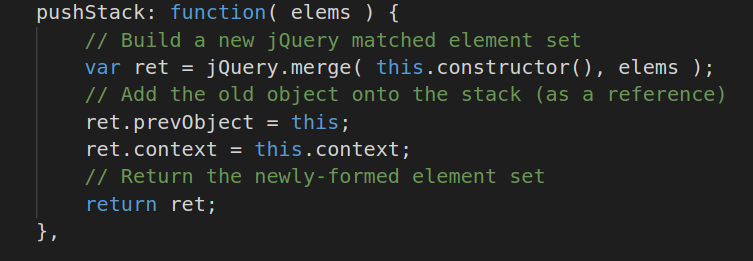
\includegraphics[width=8cm]{code_example.png} }}%
    \qquad
    \subfloat[Parsed Code Example]{\label{fig:b}{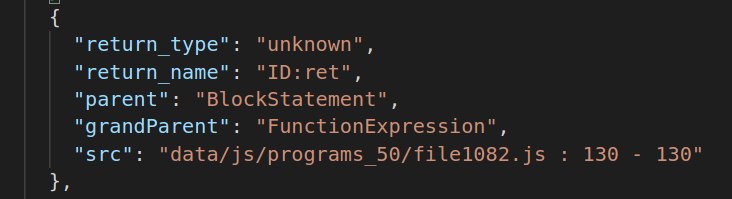
\includegraphics[width=8cm]{parsedExample.png}}}%
    \caption{Incorrect Return Statement: Parsed example using Acorn JavaScript parser}%
    
\end{figure}

\newline The next steps are to change the parsed code to vectors, prepare training data and train the model. Parsed code consists only return node, return type, parent node, and grand parent node of return argument. To convert the parsed code to vectors, all the unique nodes are defined in a separate file with a vector assigned to them. For example, node FunctionExpression has vector <0, 1, 0, 1, 0, 1, 0, 1> assigned to it. Node types are saved in a separate file and have separate vectors assigned to them. At first necessary data - return name, return type, parent, grand parent and src- are changed into vectors according to the vector values assigned to them. One one instance to vector creates only one example of a training set that is saved in a variable named $X$. There is a one more set $Y$ that saves zeros and ones where zero represent true and one represent false. Since we assume that return statement is correct in our example, we assign a $Y$ value zero to the original code example. To implement a bug, we need to change the return statement. We do so by randomly picking a return value that was used in another function in the same file. If there was no other return statement in a file, then the example is discarded. After replacing the return statement, all the inputs are changed into vectors again and saved as second entry in set $X$ created in a similar way. However, $Y$ is set to 1 this time which represents that this example is incorrect.

Sets $X$ and $Y$ together creates the training data. To generate validation data, same procedure is done on validation files that was downloaded in first step. Name the new sets $X\_validation$ and $y\_validation$ A neural network model is trained on $X$ and $y$. The input layer to the network depends upon the size of the training data. There is only one hidden layer that contains 200 neurons. The output layer produces a single number between 0 and 1 which shows the probability that a code has a particular bug. It uses activation function relu, 0.25 dropout and binary cross-entropy as a loss function. Network is trained on batch size 100 with 10 epochs. We are planning to test different activation functions such as Sigmoid, Tanh. After training, model is validated using unseen data $X\_validation$ and $y\_validation$. Model accuracy, loss and other statistics is printed out on command line. Specific examples those contain correctly predicted bug and false positives are saved in two text files namely correct.txt and anomalies.txt respectively. 


\subsection{Empty If Statement}
This bug addresses the mistake related to the empty block. Similar to Wrong Function Name bug, we traverse through the AST to find the node ConditionalExpression. If the consequent of the ConditionalExpression is type 'null' or 'undefined', then we have successfully spotted an empty if statement. For each call, this approach extracts the following information:
\begin{enumerate}
    \item The kind of AST node parent and grand-parent nodes 
    \item The name and type of the consequent if there is any
\end{enumerate}
Extracting parent and grandparent help in obtaining some context about the area where the problem is found. We look through each conditional expression and check the value and type of their consequents. An empty consequent would have a type 'null' and no entry for the name field(since it is empty). We also consider cases where the name field contains an entry 'ID: undefined' and type as 'undefined'.  

 \newline Here we look for conditional expressions  and check the nature of their consequents(name, type and other properties).  We have used the file extractorOfConditional to accomplish this. This produces two text files . Figure 5 illustrates how this parsing is done. The first file acts as the training set while the second file helps in checking the validity of our model. The parsed code is then translated to to its corresponding vector and we train the model. Parsed code consists of consequent name, consequent type, parent node, and grand parent node of the conditional expression. \newline
\begin{figure}[!htb]
    \centering
    \subfloat[Code Example  ]{{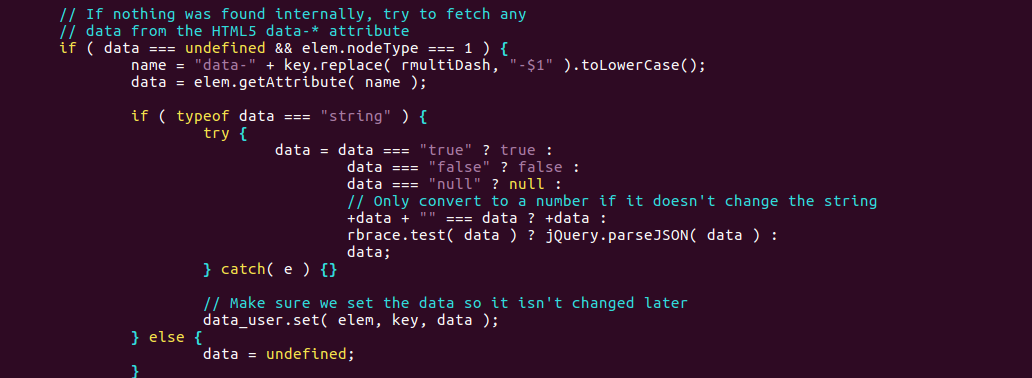
\includegraphics[width=8cm]{code_example2.png} }}%
    
    \qquad

    \subfloat[Parsed Code Example ]{{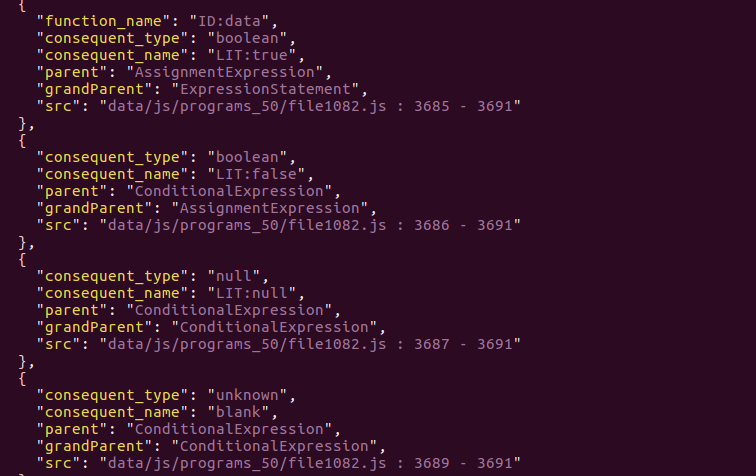
\includegraphics[width=8cm]{parsedExample2.png} }}%
    \caption{Incorrect Conditional: Parsed example using Acorn JavaScript parser}%
    \label{accuracy_and_loss_incorrect_if_statement}%
\end{figure}
\newline Similar to Incorrect Return Statement, each component of the extracted information in the parsed file is mapped to its corresponding vector. For example, a consequent of type boolean is found to have a corresponding type vector <1, 1, 0, 1, 0>. Vectors are assigned to each unique node and each instance is referred to using the variable X while the variable Y denotes the class(containing zero or one values) that indicates whether the code belongs in the 'non-buggy' class or 'buggy' class(as indicated in Figure 6).
\newline A negative example is generated by performing a simple transformation in a file. We simply replace the consequent of the picked conditional expression with a random null or undefined value (thus creating buggy code). After doing this we translate the inputs into vectors again but set the Y to 1 indicating that this is a negative(buggy) example. Together X and Y constitute the data for training. The same technique is repeated on the validation files prepared in the parsing step to obtain the validation dataset. The same neural network(as was used for Incorrect Return statement) is trained on X and Y with batch size 100 and 10 epochs.
\begin{figure}[h!]
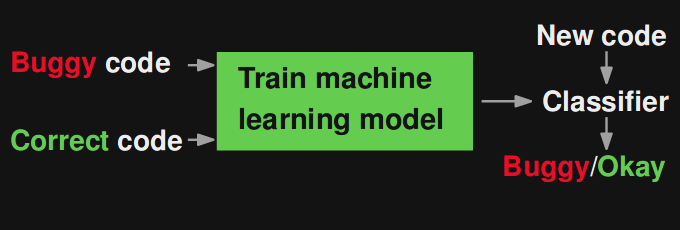
\includegraphics[width=50mm]{untitled(3).png}
\caption{Training a model to identify instances of bug patterns\cite{slidepradel}}
\end{figure}
\newline After training is complete, the model needs to be validated on unseen data $X\_validation$ and $y\_validation$ to obtain the measures of model accuracy, loss and other statistics. Similar to Incorrect Return Statement, we save discrete examples of successful predictions into correct.txt while storing the false positive instances in anomalies.txt. 
An example of a conditional expression that also satisfies the criterion of being an empty block is the one in Figure \ref{correct conditional}. As is evident from the Figure, the conditional expression executes a null expression if true(which is equivalent to executing an empty block).
\begin{figure}[!ht]
  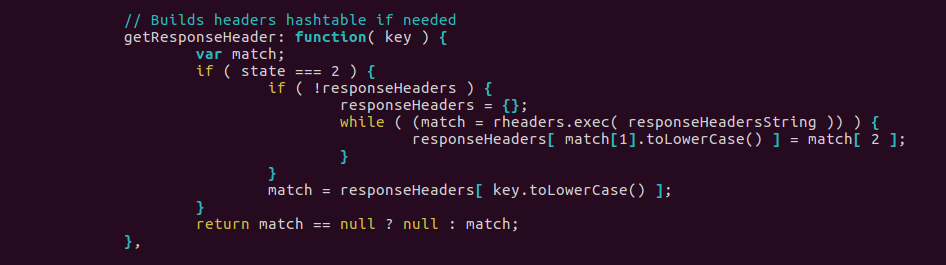
\includegraphics[width= \linewidth]{correct conditional.png}
  \caption{\small Empty block in Conditional expression}\label{correct conditional}
\end{figure}

\section{Evaluation}
Newly trained models are evaluated on both small corpus and big corpus. Our major evaluation questions are:

\begin{enumerate}
\item Can newly trained models effectively find bugs?
\item How useful are the trained Bug Detectors (what is the accuracy of our model) ?
\item How much time it takes to train the model (Efficiency) ?
\end{enumerate}



\subsection{Finding Bugs}
To evaluate our models, the first question is whether or not models can distinguish between buggy and correct code. During evaluation of model, we outputs two files, namely correct.txt and anomalies.txt. Like their names, correct.txt provides examples of correctly predicted bug, and anomalies.txt provided examples of false positives and false negatives. Correct.txt reported that one of the correctly predicted example exist in File 1082 with Line457. This specific code example is shown in Figure \ref{fig:incorrect example}. Model Correctly predicted that returned keyword 'matches' is correct instead of keyword  'length' that it was replaced with. 
%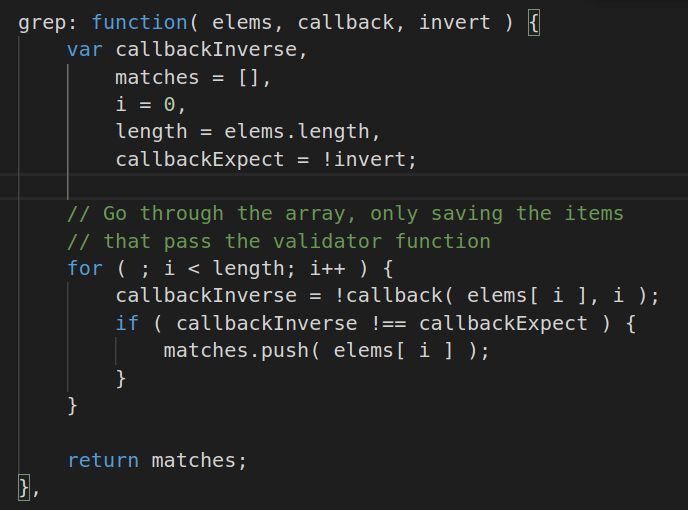
\includegraphics[width= 9cm]{correctly predicted example return statement.png}

  \begin{figure}[!ht]    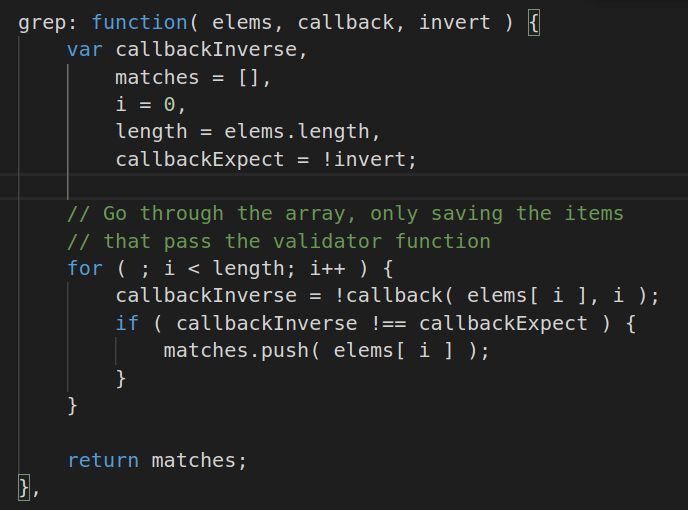
\includegraphics[width=\linewidth]{correctly predicted example return statement.png}
    \caption{Example}\label{fig:incorrect example}
  \end{figure}

One entry from anomalies file- that model predicted wrong- is File 1082, L7599. This example is shown in Figure \ref{false positive} Model falsely predicted that the given return statement is a bug. This is an example of a false positive. 

%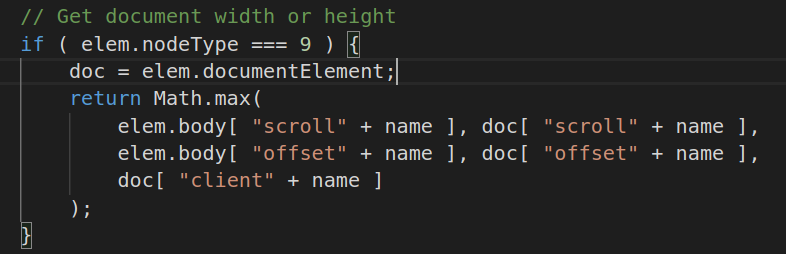
\includegraphics[width= 9cm]{return_statment Predicted Wrong.png}


\begin{figure}[!ht]
  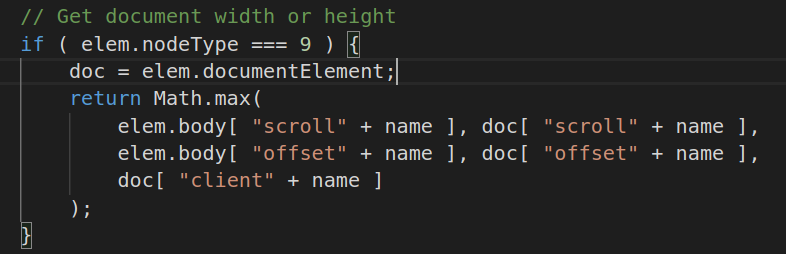
\includegraphics[width= \linewidth]{return_statment Predicted Wrong.png}
  \caption{\small Incorrect Return Statement Bug Detector- False Positive}\label{false positive}
\end{figure}


 
\subsection{Accuracy}
We have divided the code examples into two sets, training examples and validation examples. After training the model, validation examples are fed to the model. Model produces accuracy, recall and precision score once we compare the generated output to the correct output. Accuracy score tells how many times the model spotted the bug correctly. Simple accuracy score is the first criteria to evaluate our model. More accuracy, model has, better it is to predict the specific bug that it has been trained on. Figure \ref{fig:accuracy_and_loss_incorrect_return_statement} shows how model accuracy was improved and loss was minimized during training. Table \ref{tab:my_label} shows the accuracy, precision, and recall results of both trained models. The small corpus gave only 50\%accuracy in both models. However, after training the model on big corpus, we got 71\% accuracy on Incorrect Return Statement Bug Detection. The accuracy is not very impressive; however, it would still help in spotting bugs related to wrong return statement. Empty Block Statement Bug Detection provides 91\% accuracy which is compatible with the accuracy of swapped args, wrong binary operand and wrong binary operator bug detection those were reported by DeepBugs paper originally. Precision and Recall were also improved with large corpus compare to smaller one. 

\begin{figure}[!htb]
    \centering
    \subfloat[Training and Validation Accuracy ]{{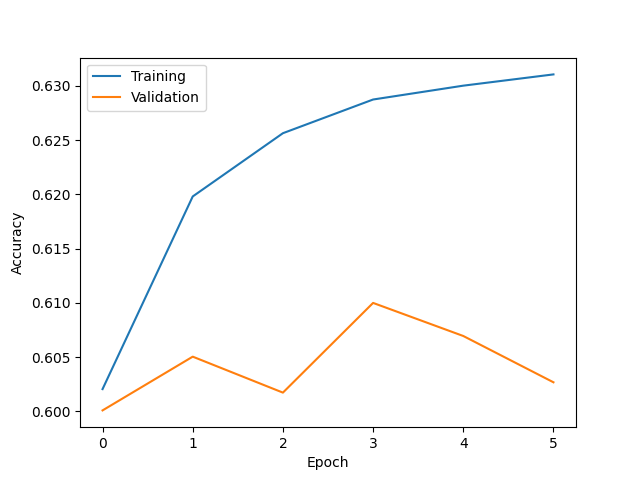
\includegraphics[width=8cm]{accuracy_graph_IncorrectReturnStatement.png} }}%
    \qquad
    \subfloat[Training and Validation Loss ]{{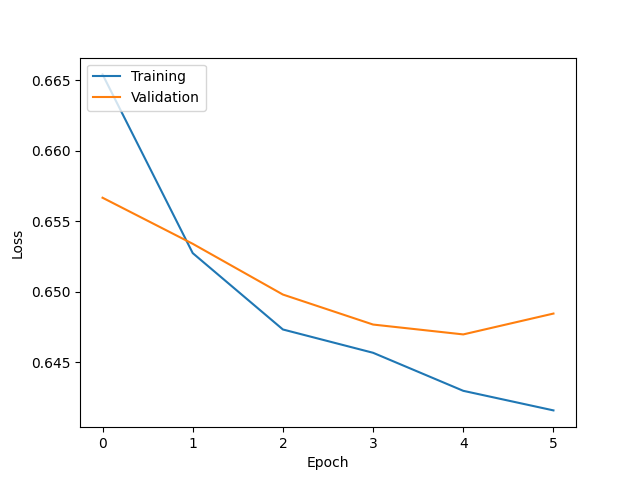
\includegraphics[width=8cm]{loss_graph_IncorrectReturnStatement.png} }}%
    \caption{Accuracy and Loss of Incorrect Return Statement Bug Detector Model }%
    \label{fig:accuracy_and_loss_incorrect_return_statement}%
\end{figure}


  
\begin{table}[h!]
    \centering
    \begin{tabular}{l ccc}
        \hline
        Bug Detector & Accuracy & Precision & Recall\\
        \hline
        \hline
        Corpus of 50 files & & & \\
        \cline{1-1}
        Wrong Return Statement & 0.50 & 0.81 & 0.29 \\
        Empty Block Statement & 0.50 & 0.04 & 0.1 \\
        \hline
        Corpus of 150,000 files & & & \\
        \cline{1-1}
        Wrong Return Statement & 0.71 & 0.82 & 0.60 \\
        Empty Block Statement & 0.91 & 0.81 & 1.0 \\
        \hline
    \end{tabular}
    \caption{Final Result Accuracy}
    \label{tab:my_label}
\end{table}  



\iffalse
\begin{figure*}[!htb]
 \centering
  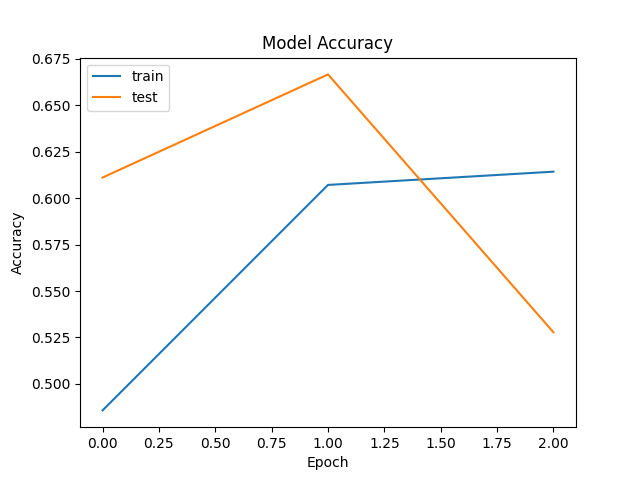
\includegraphics[width=0.5\textwidth]{accuracy_graph_IncorrectReturnStatment.png}
  \caption{\small Accuracy Graph- Incorrect Return Statement}
\end{figure*}

\begin{figure*}[!htb]
 \centering
  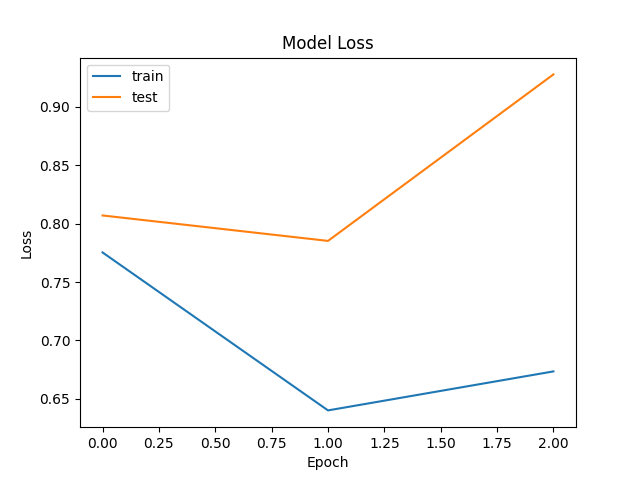
\includegraphics[width=0.5\textwidth]{loss_graph_IncorrectReturnStatment.png}
  \caption{\small Loss Graph- Incorrect Return Statement}
\end{figure*}

\fi

\subsection{Efficiency}
In this section, we evaluate how fast the model runs. Training time consists of the time it is used to extract the code examples and train a classifier. Prediction time consist of time it takes to extract the previously unseen code examples and the time that trained model takes to predict an output. On small corpus, our model did not take much long. However, on large corpus with 150,000 files, extraction took about 30 minutes and training took five minutes. Training a model with 2,168,944 examples in five minutes is impressive. Time taken also may depend upon the machine that you ar training the model on. Hence, varied results for time consumption are expected. Machine that the experiments were run have following specifications: Intel Core i7 Processor and 16GB RAM. Full results are shown in Table \ref{tab: time_table}. 


\begin{table}[h!]
\begin{tabular}{l cc | cc}
\toprule
Bug Detector & \multicolumn{2}{c}{Training} & \multicolumn{2}{c}{Prediction} \\
%\cline{2-6} \cline{8-12}
\cline{2-5}
 & Extract & Learn & Extract & Predict \\
\midrule
\hline
Corpus of 50 files & & & \\
\cline{1-1}
Wrong Return Statement  & 00:05 & 00:09 & 00:03 & 00:02 \\
Empty Block Statement & 00:04 & 00:05 & 00:02 & 00:02 \\
\hline
Corpus of 150,000 files & & & \\
\cline{1-1}
Wrong Return Statement  & 25:19 & 05:07 & 12:18 & 04:06 \\
Empty Block Statement & 20:05 & 12:98 & 16:07 & 08:08 \\
\bottomrule
\end{tabular}
\caption{Time (mm:ss) Taken for Training}
\label{tab: time_table}
\end{table} 


\section{Contribution}
Our work contributes to the DeepBugs paper to handle two more bugs, wrong return statements and empty block statement. We used the same algorithm that DeepBugs have used. To convert the corpus to desired format, we added two files name extractorOFRetVal.js and extractorOfConditional.js for both two bugs. To create a training data for Wrong Return Statment, we added LearningDataReturnStatement.py and for empty block statment, we added LearningDataIfStatement.py.   

Lakhveer and Iman did equal amount of work. From two newly added bugs, Lakhveer worked on wrong return statement, and Iman worked on empty if blocks. Both bugs are at the same level, where we have extracted the code snippets into vector format.
The current version of the working code has been pushed to a branch named imanbranch on the repo. Iman did the pushing and tested all the javscript files while Lakhveer studied the python files.The data being used in the Deepbugs project is used as our data source. The corpus used contains 100,000 JavaScript training files and a validation set of 50,000 JavaScript files( JS150 corpus available at ). In total, the corpus amounts to 68 million lines of code. For the current analysis we have performed a preliminary test on a much smaller corpus of  50 programs provided by the authors.

\section{Conclusion}

We have applied our framework on the large corpus of 150,000 files and added two bug detectors to the existing system . We obtain very promising accuracies of
71\% and 91\% respectively for the bugs Incorrect Return Statement and Empty Block and obtain a sizeable improvement over the performance of 50\% obtained with the small 50-file corpus. We believe that our work will be very useful to substitute for the human effort involved in detecting bugs. We also expect our model to utilize the information learnt from existing code to complement manually designed bug detectors. This is highly appropriate for software systems that are sensitive to unpredictable faults arising from carelessly coded corner cases. If not for the time constraint, we could have been able to improve the prediction accuracy further.

%%
%% The next two lines define the bibliography style to be used, and
%% the bibliography file.
\bibliographystyle{plain}
\bibliography{references}

\end{document}
\endinput
%%
%% End of file `sample-sigconf.tex'.
